\vspace{-0.4cm}
\textit{``Em pleno 2022; ano da tecnologia; ano da
eleição; ano da copa; ano em que empresários bilionários estão construindo
    foguetes; neste ano, é
necessário malhar bastante na academia''}. Com essa filosofia em mente, Gustavo vai
à academia treinar todos os dias depois do trabalho.

Diversos exercícios da academia envolvem encaixar anilhas (pesos em forma de
disco) nas duas pontas de uma barra de ferro, para então erguer a barra em uma
posição que favorece determinado músculo.
Para que o exercício seja executado corretamente, é necessário que o peso total
em uma ponta da barra seja igual ao peso total na outra ponta da barra, como no
exemplo abaixo:

\vspace{-0.4cm}
\begin{center}
    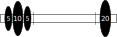
\includegraphics[scale=0.5]{pesos/pesos.png}
\end{center}

\vspace{-0.5cm}
Gustavo quer treinar o máximo possível e, por isso, quer usar
\textit{todas} as anilhas disponíveis na academia.
Dadas as anilhas disponíveis e seus pesos, é possível distribuir \textit{todas}
as anilhas nas duas pontas da barra de forma que o peso total seja o mesmo em ambas?

\subsection*{Entrada}

A primeira linha contém o inteiro $N$ ($1 \leq N \leq 100$), o número de
anilhas disponíveis. A segunda linha contém $N$ inteiros $P_i$ ($1 \leq P_i \leq 100$), o
peso de cada anilha, em quilogramas.

Considere que a barra é comprida o bastante de forma que é possível colocar
qualquer quantidade de anilhas, em ambas as pontas.

\subsection*{Saída}

Imprima uma única linha contendo \verb|SIM| se é possível distribuir todas as
anilhas nas duas pontas da barra de forma que o peso total seja o mesmo em
ambas, ou \verb|NAO| caso contrário.

\begin{table}[!h]
\centering
\begin{tabular}{|l|l|}
\hline
\begin{minipage}[t]{3in}
\textbf{Exemplo de entrada}
\begin{verbatim}
4
5 20 5 10
\end{verbatim}
\vspace{1mm}
\end{minipage}
&
\begin{minipage}[t]{3in}
\textbf{Exemplo de saída}
\begin{verbatim}
SIM
\end{verbatim}
\vspace{1mm}
\end{minipage} \\
\hline
\end{tabular}
\end{table}

\begin{table}[!h]
\centering
\begin{tabular}{|l|l|}
\hline
\begin{minipage}[t]{3in}
\textbf{Exemplo de entrada}
\begin{verbatim}
3
20 5 10
\end{verbatim}
\vspace{1mm}
\end{minipage}
&
\begin{minipage}[t]{3in}
\textbf{Exemplo de saída}
\begin{verbatim}
NAO
\end{verbatim}
\vspace{1mm}
\end{minipage} \\
\hline
\end{tabular}
\end{table}

\begin{table}[!h]
\centering
\begin{tabular}{|l|l|}
\hline
\begin{minipage}[t]{3in}
\textbf{Exemplo de entrada}
\begin{verbatim}
6
5 5 10 10 15 15
\end{verbatim}
\vspace{1mm}
\end{minipage}
&
\begin{minipage}[t]{3in}
\textbf{Exemplo de saída}
\begin{verbatim}
SIM
\end{verbatim}
\vspace{1mm}
\end{minipage} \\
\hline
\end{tabular}
\end{table}
